\documentclass{article}
\usepackage[utf8]{inputenc}
\usepackage{algpseudocode}
\usepackage{algorithm}
\usepackage{tikz}
\usepackage{amsmath}
\usepackage{amssymb}
\usetikzlibrary{automata}
\setcounter{MaxMatrixCols}{25}

\title{Algorithmique Avancée TD02}
\author{Hugo Demaret}
\date{September 2021}
\begin{document}
\maketitle
\section*{Exercice 1.3 -}
\textit{Montrez que tout groupe d'au moins deux personnes contient toujours au moins deux individus ayant le même nombre d'amis.}\\
\textsf{Cas trivial du groupe à deux personnes :}\\
\textsf{Si connexe : 1 ami, sinon 0}\\
\textsf{Le graphe possède n sommet, et k arêtes.}\\
\textsf{On procède par récurrence :}
    \begin{center}
        $
            \textrm{On utilise le lemme des tiroirs :}
            \linebreak
            \textrm{On a n sommet, et au plus n-1 étiquette.}
            \linebreak
            \textrm{Par principe des tiroirs, au moins deux sommets on la même etiquette.}
        $
    \end{center}
\section*{Exercice 1.4 -}
    \textit{Soit $(d_{1},...,d_{n})$ la suite des degrés d'un graphe non-dirigé G.}\\
    \textit{On note $\delta(G)$ et $\bigtriangleup(G)$ respectivement le plus petit et le plus grand de ces sommets.}\\
    \subsection*{1 -}
        \textit{Montrez que $\sum_{i=1}^{n} di = 2m(G) $.}
            \begin{center}
            $
            \textit{Quand on ajoute une arête, on augmente le degré de deux sommets.}
            \linebreak
            \textit{La somme des degrés du graphe vaut n, et deux fois plus de sommets. D'ou :}
            \linebreak
            \sum_{i=1}^{n} di = 2m(G) 
            $
            \end{center}
    \subsection*{2 -}
            \textit{En déduire que $\delta(G) \leq \frac{2m(G)}{n(G)} \leq \bigtriangleup(G)$}\\
            \begin{center}
            $
            \forall i \in \{1,...,n\} \delta(G) \leq d_{i} \leq \bigtriangleup(G)
            \linebreak
            \Rightarrow \sum_{i=1}^{n} \delta(G) \leq \sum_{i=1}^{n} d_{i} \leq \sum_{i=1}^{n} \bigtriangleup(G)
            \linebreak
            \Rightarrow n \delta(G) \leq 2m(G) \leq n\bigtriangleup(G)
            \linebreak
            \Rightarrow  \delta(G) \leq \frac{2m(G)}{n(G)} \leq \bigtriangleup(G)
            $
            \end{center}
\section*{Exercice 1.5 -}
\textit{Le but de cet exercice est de montrer que deux plus longs chemins dans un graphe\\ non-orienté connexe G ont forcément un sommet commun.}
    \subsection*{1 -}
            \textit{Si les deux chemins ont la même longueur :}
            \linebreak
            \textit{- Soit ils partent du même sommet (ou arrivent au même) et sont joints.}
            \linebreak
            \textit{- Soit ils ne partent pas du même sommet (et n'arrivent pas au même sommet).}
            \linebreak
            \textit{On peut donc couper le graphe en deux sous graphes}
            \linebreak
            \textit{Pour chacun de ces deux sous graphes, on ne considère que les chemins.}
            \linebreak
            \textit{Ces sous graphes sont alors homéomorphe à un segment.}
            \linebreak
            \textit{La distance étant égale, on peut tracer deux cordes}
            \linebreak
            \textit{(les deux chemins) sur un cercle de rayon k, avec k étant le nombre de sommets}
            \linebreak
            \textit{Ces deux cordes sont en fait des rayons, car de longueur k.}
            \linebreak
            \textit{Deux rayons d'un cercle s'intersectent toujours.}
            \linebreak
            \textit{Donc les deux chemins se croisent. Absurde.}
    \subsection*{2 -}
        \textsf{Étant donné que les deux chemins se croisent (car non-disjoints), il existe au moins un sommet en commun.}
    \subsection*{3 -}
        \textsf{Dans le cas d'un graphe non-connexe nom : graphe composé de deux fois un même sous graphe.}
        \textsf{Dans le cas d'un graphe orienté faiblement connexe, cette propriété est fausse :}
        \begin{center}
            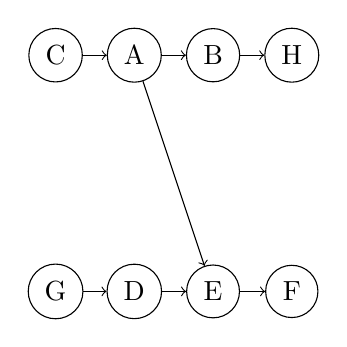
\begin{tikzpicture}
                \node[circle,draw=black](A) at(0,0) {A};
                \node[circle,draw=black](B) at (1,0) {B};
                \node[circle,draw=black](C) at (-1,0) {C};
                \node[circle,draw=black](H) at (2,0) {H};
                \node[circle,draw=black](D) at (0,-3) {D};
                \node[circle,draw=black](E) at (1,-3) {E};
                \node[circle,draw=black](F) at (2,-3) {F};
                \node[circle,draw=black](G) at (-1,-3) {G};
                \draw[->](C)--(A);
                \draw[->](A)--(B);
                \draw[->](B)--(H);
                \draw[->](E)--(F);
                \draw[->](D)--(E);
                \draw[->](G)--(D);
                \draw[->](A)--(E);
            \end{tikzpicture}
        \end{center}
\end{document}